\section{Memory analysis}
In this section it will be explained how the SMB buffers are stored in the Windows systems. This is very important in order to know 
what the attacker is overflowing and how he can be able to execute the code.\\
At the end of the section ther will be a short overview about the grooming technique, a procedure to predict where is the next memory alocation.
\subsection{Srvnet buffers}
A srvnet buffer is a struct used to store the content of smb transactions, it is composed by three components:
\begin{itemize}
    \item srvnet\_wsk\_struct: It contains a table of functions pointers, they are executed by the server machine in some specific occasion, for example
    when the connection is stopped it executes the function SrvNetWskReceiveComplete() to process the data in the buffer.
    \item Memory Description List (MDL): A kernel structure that maps the data buffer to the physical memory fragments.
    \item The buffer data itself
\end{itemize}

\begin{figure}[ht!]
    \centering
      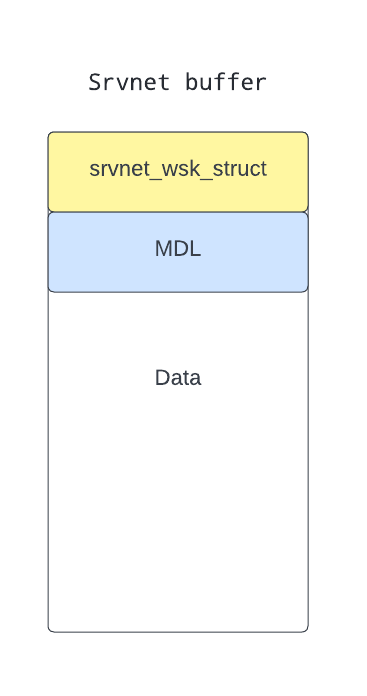
\includegraphics[scale=0.7]{images/srvnet_buffer.png}
      \caption{Srvnet buffer}
\end{figure}

\clearpage

\subsection{Hal's Heap}
The Windows Hardware Abstraction Layer (HAL) is a module that runs in kernel mode and it is loaded on Windows boot. It consists in a set of routines to access hardware resources
through programming interface. This is used to allow programmers to write software which is hardware-indipendent.\\
This is a particular heap in Windows, its addres has been kept always costant. The Address Space Layout Randomization (ASLR), which consists in the randomization of the memory addresses,
doesn't regards the ones in the HAL heap which are always costant.
Fortunately, in the last versions of Windows 10 also the HAL's heap is randomized, but not at the time of the exploit.
Another important feature of the HAL's heap is that it has execution permission is some Windows version.\\
It is clear now that this part of memory is perfect for the exploitation, here is where the attacker wants to execute the payload.

\begin{figure}[ht!]
    \centering
      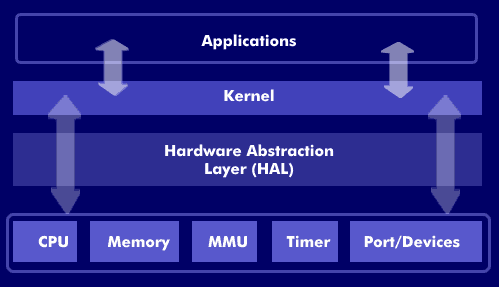
\includegraphics[scale=0.5]{images/hal.png}
      \caption{Hardware description layer}
\end{figure}

\clearpage

\subsection{Grooming technique}
If the attacker wants to use a buffer overflow as a remote code execution, he has to control the memory that he is overwriting. There are many ways to do it, in 
the case of EternalBlue this is done by the grooming technique. This method is based on the concept that the memory allocations tend to reuse the same chunks of memory. So if the 
attacker allocates a buffer of X bytes and the free it, it is very probable that if he does another malloc() of X bytes it will be stored in the same location.\\
Thanks to that, the attacker can predict the location where the buffer will be stored by creating a custom-sized memory and free it just before he needs to store the new buffer. In the case of 
EternalBlue this technique will be used by doing a small heap allocation with secondary transaction and a custom-sized heap allocation with the vulnerabilty explained in 3.3
The following images shows the passages used for this technique.

\begin{figure}[ht!]
    \centering
      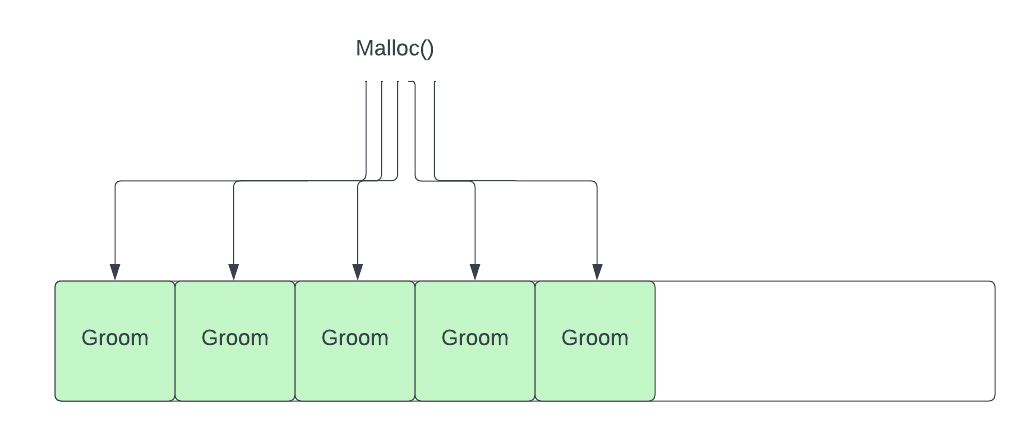
\includegraphics[scale=0.5]{images/grooming_malloc.png}
      \caption{Hardware description layer}
\end{figure}

\begin{figure}[ht!]
    \centering
      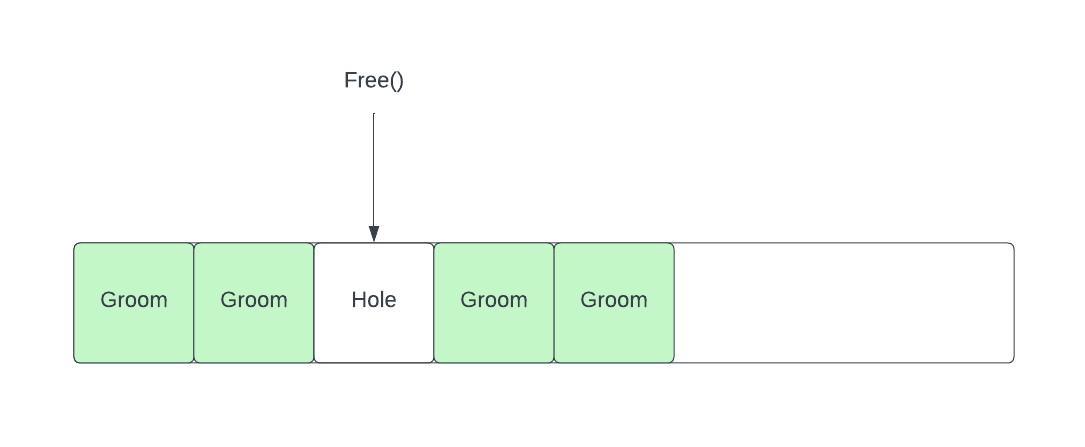
\includegraphics[scale=0.5]{images/grooming_free.png}
      \caption{Hardware description layer}
\end{figure}

\begin{figure}[ht!]
    \centering
      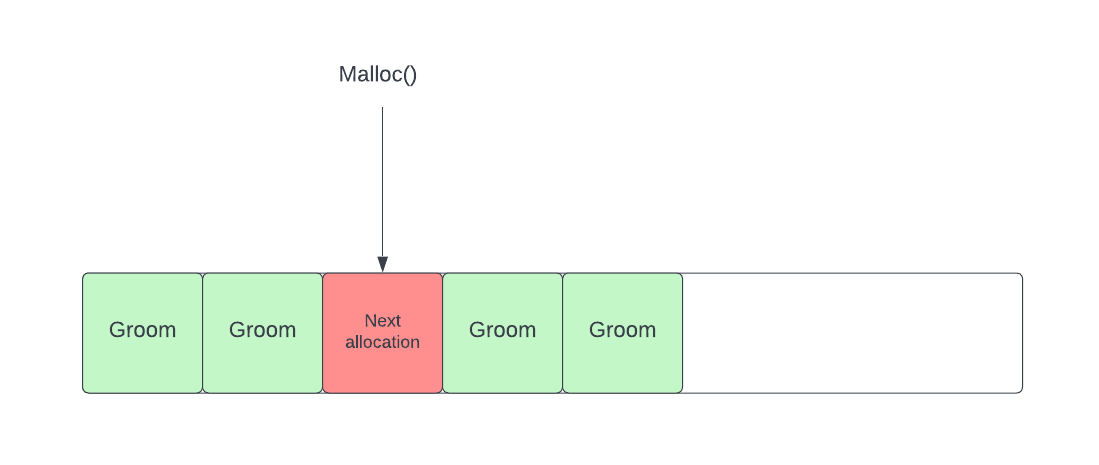
\includegraphics[scale=0.5]{images/grooming_prediction.png}
      \caption{Hardware description layer}
\end{figure}